
We present in this chapter the different case studies used along the thesis. We consider models from different sources with varying size. 
Our models are: 
%
the soda vending machine model (\textit{S. V. Mach.}) in Section \ref{sec:casestudy:svm};
%
the mine pump (\textit{Mine\-pump}) in Section \ref{sec:casestudy:minepump};
%
the WordPress models (\textit{AGE-RR}, \textit{AGE-RRN}, \textit{Elsa-RR}, and \textit{Elsa-RRN}) in Section \ref{sec:casestudy:wordpress};
%
the Claroline website (\textit{Claroline}) in Section \ref{sec:casestudy:claroline};
%
and the random models (\textit{Random} \textit{1-4}) in Section \ref{sec:casestudy:random}.
%
We compare the models characteristics in Section \ref{sec:casestudy:characteristics} and define the threats to validity linked to the selection of our case studies in Section \ref{sec:casestudy:threats}.


%%%%%%%%%%%%%%%%%%%%%%%%%%%%%%%%%%%
\section{Soda vending machine}
%%%%%%%%%%%%%%%%%%%%%%%%%%%%%%%%%%%

\label{sec:casestudy:svm}

\begin{figure}[t]
	\centering
	\subbottom[Feature model]{
		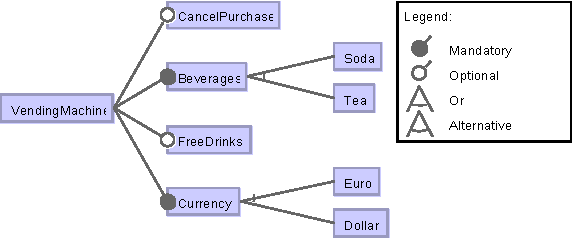
\includegraphics[width=95mm]{svm-fm}
		\label{fig:svmfm}
	}	
	\subbottom[Featured transition system]{
		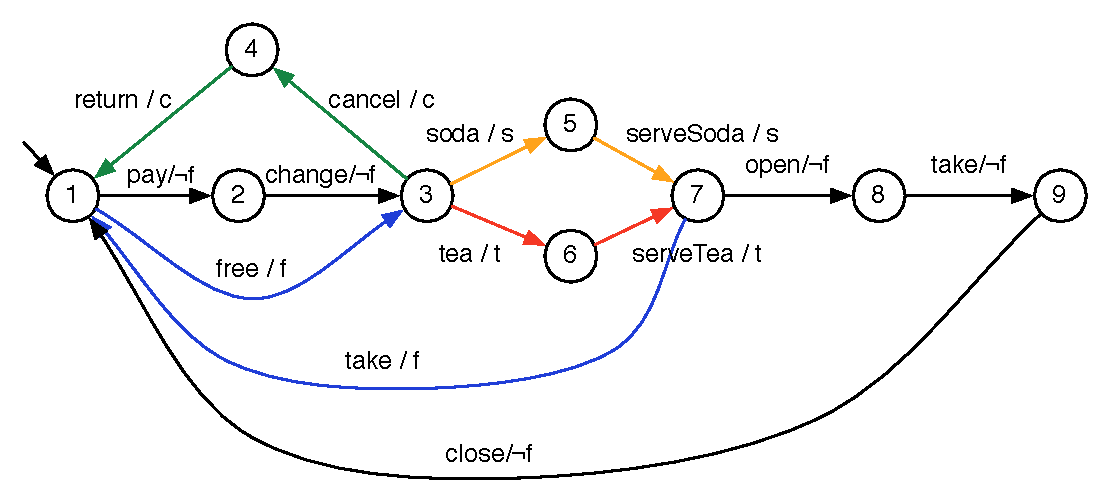
\includegraphics[width=105mm]{svm-fts}
		\label{fig:svmfts}
	}
	\caption{Soda vending machine}
\end{figure}

The \gls{soda vending machine} SPL is a classical beverage vending machine described by Classen \etal \cite{Classen2013b}. The \gls{feature model} is presented in Figure \ref{fig:svmfm}: it sells soda ($s$) or tea ($t$) in euro or dollar, may offer free drinks ($f$), and optionally allows to cancel a purchase ($c$). The \gls{FTS} describing the behaviour of the SPL is presented in Figure \ref{fig:svmfts} (for readability, the feature names have been shortened): the user either pays or chooses a free drink (if feature $f$ has been selected); he may cancel its purchase (if feature $c$ has been selected); he chooses a beverage, allowed by the selected features; and gets his beverage directly (if feature $f$ has been selected) of after opening the machine (otherwise).


%%%%%%%%%%%%%%%%%%%%%%%%%%%%%%%%%%%
\section{Card payment terminal}
%%%%%%%%%%%%%%%%%%%%%%%%%%%%%%%%%%%

\label{sec:casestudy:cpterminal}

\begin{figure}
	\centering
	\subbottom[Feature model]{
		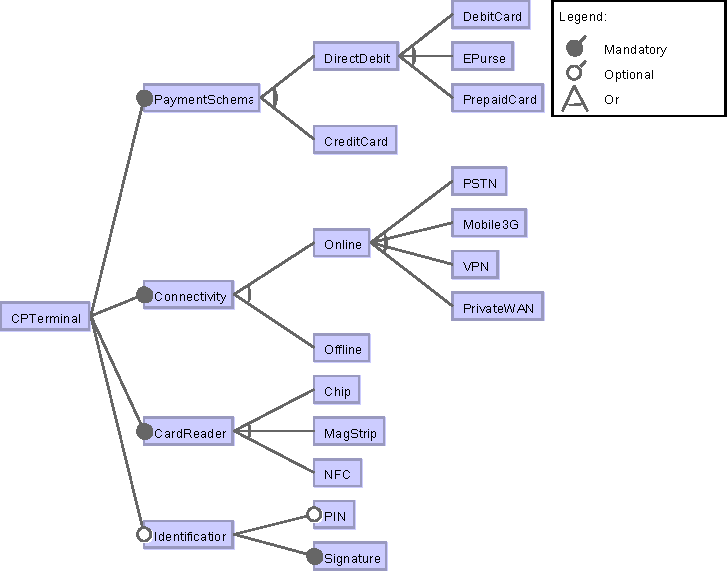
\includegraphics[width=110mm]{cpterminal-fm}
		\label{fig:cpterminalfm}
	}	
	\subbottom[Featured transition system]{
		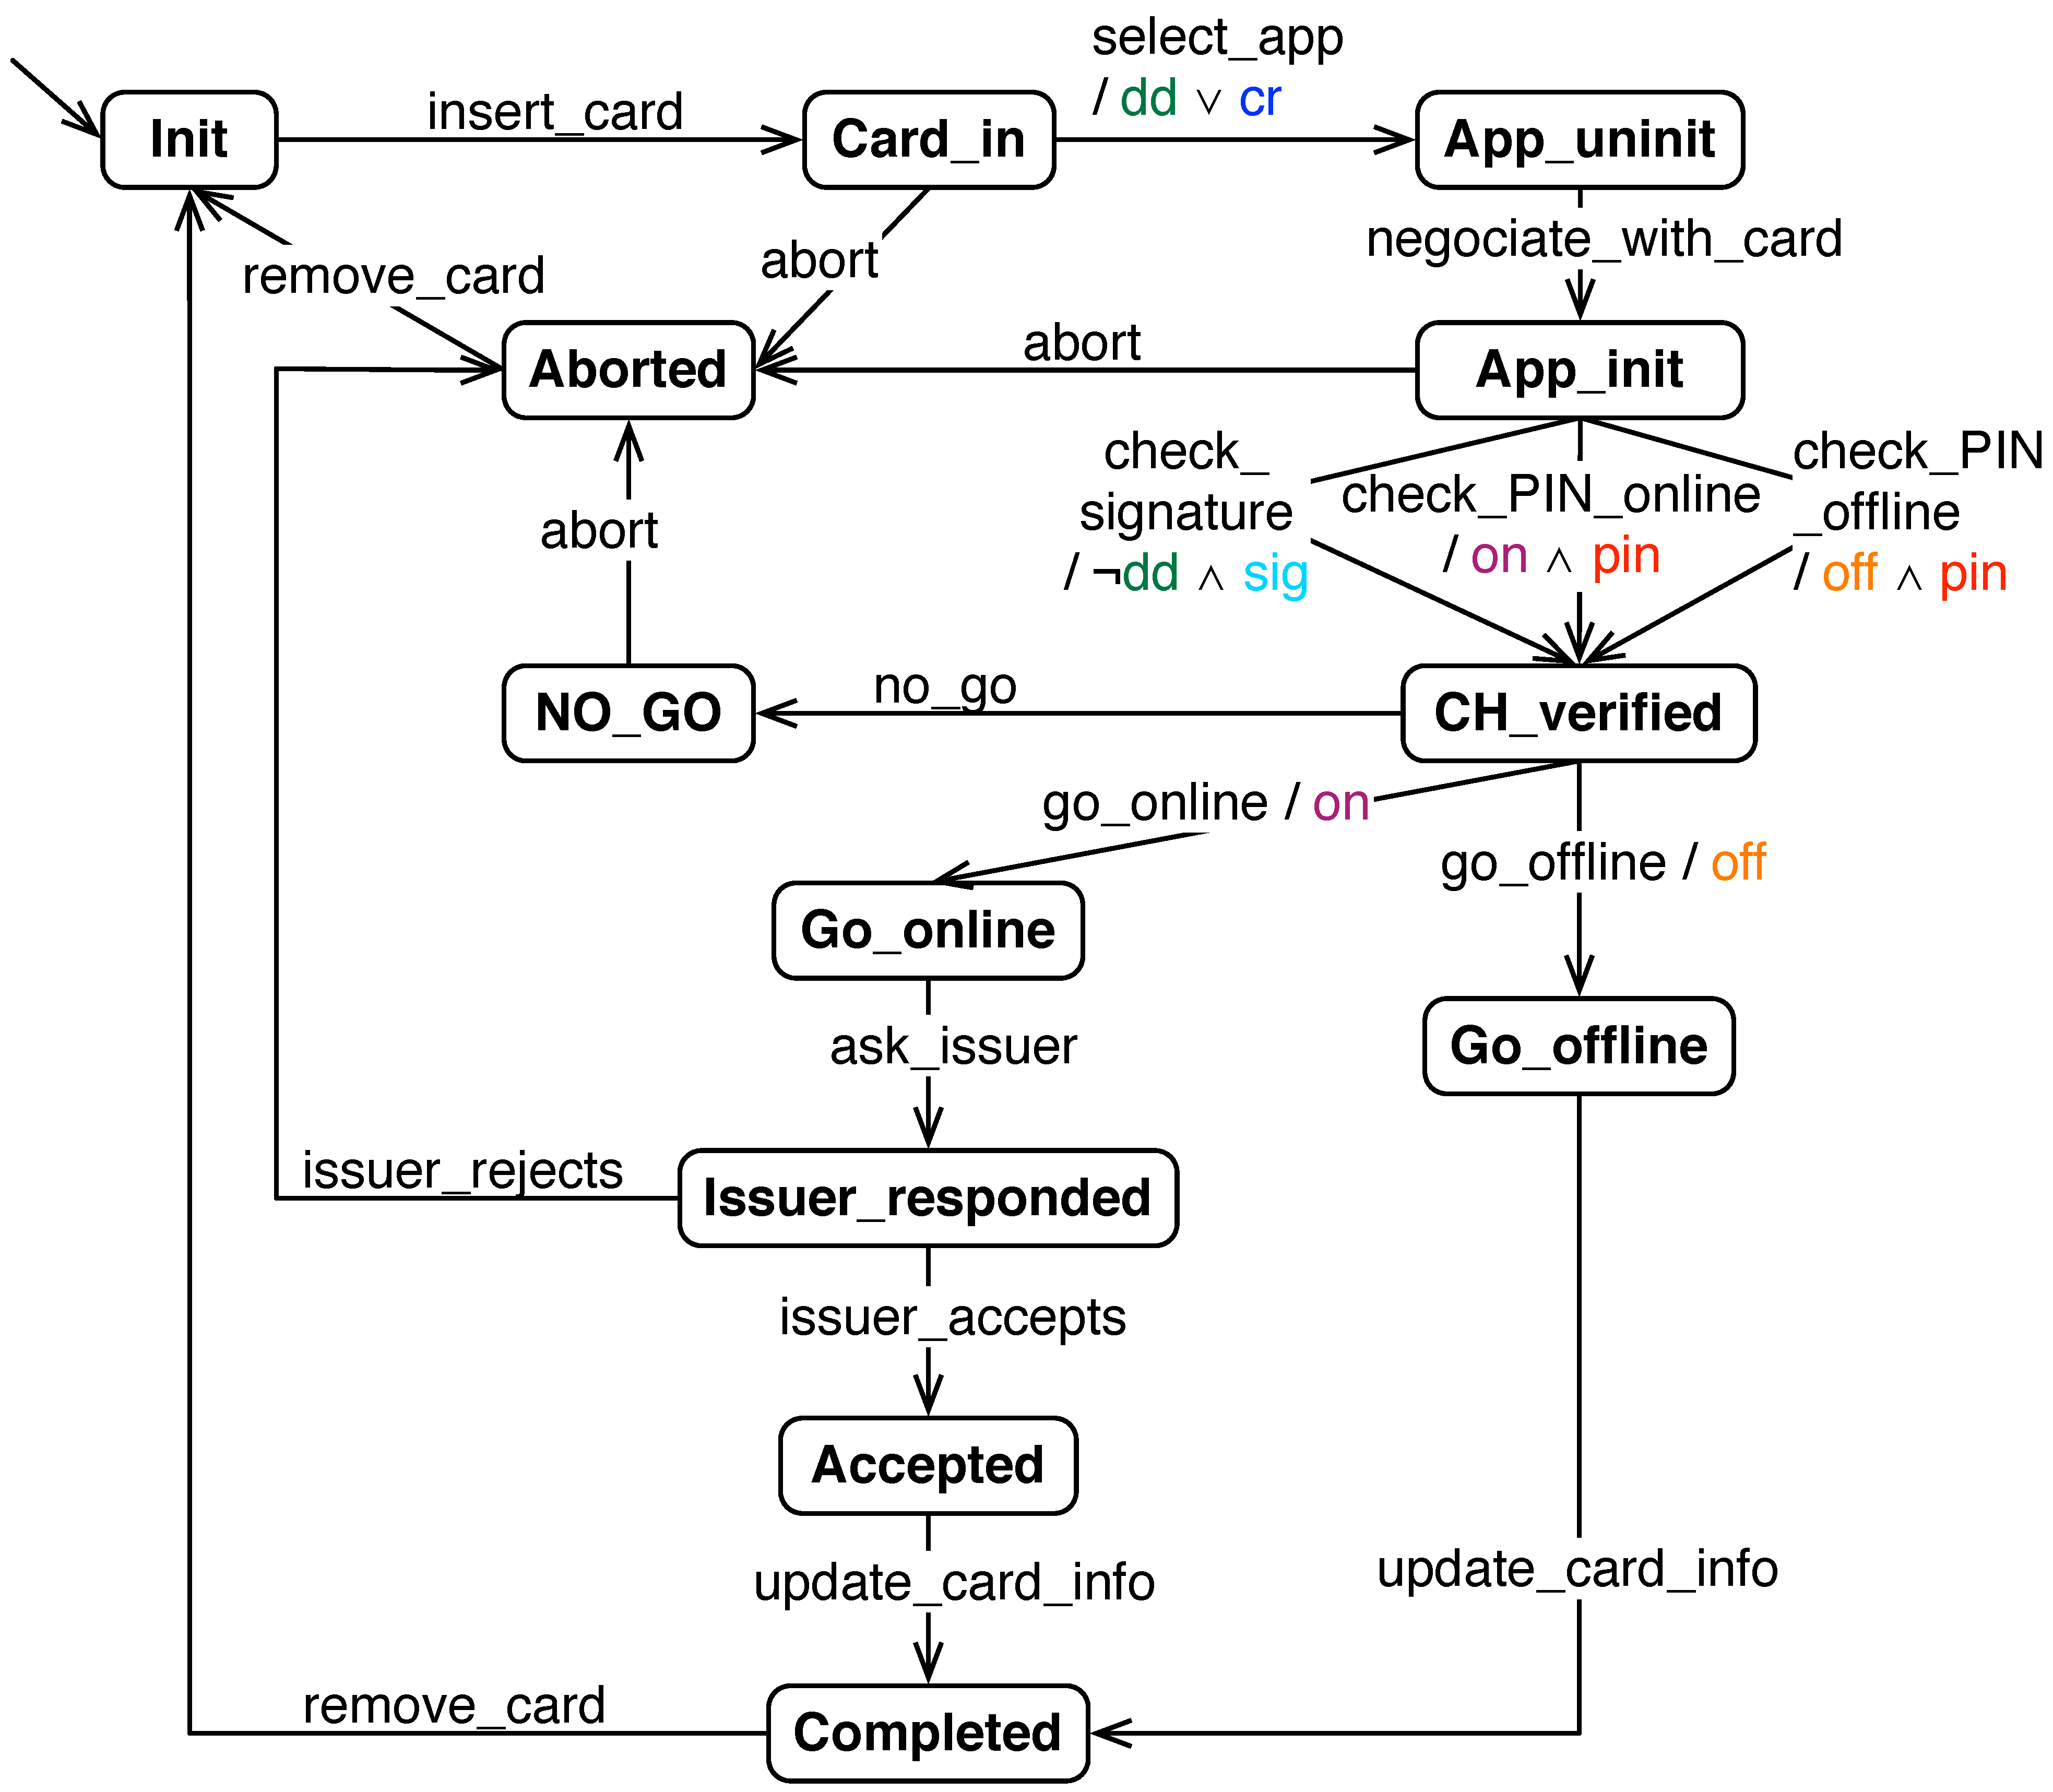
\includegraphics[width=85mm]{cpterminal-fts}
		\label{fig:cpterminalfts}
	}
	\caption{Card payment terminal}
\end{figure}

Figure \ref{fig:cpterminalfm} presents the \gls{feature model} of a card payment terminal manually defined using Eurocard-Mastercard-Visa (EMV) specification document \cite{EMVCo2011}. This machine accepts card payment with a given payment schema (direct debit and/or credit card). It works online, using one or more connectivity option, or offline with the card payment service. Cards are read using a chip, the magnetic strip, or near field contact (NFC); and card owner may be authenticated using signature and optionally PIN code.

The FTS in Figure \ref{fig:cpterminalfts} presents the behaviour (we want to test) of the card payment terminal (minus one technical intermediate state) to processes a payment. First, the Card Holder (CH), \ie the user, inserts his card in the terminal. If the card is a direct debit ($dd$) or a credit card ($cr$), the terminal will proceed the initialisation of the transaction. In this version of the product line, the card holder must always identify himself using either: his signature if the card is not a direct debit card and if the terminal supports the signature identification ($sig$); or his secret \gls{PIN} if the terminal supports PIN identification ($pin$), which may be checked online ($on$) or offline ($off$) with the transaction processor company. If the identification succeeds, the terminal will proceed online or offline to the payment, otherwise, the transaction is aborted. Whether the transaction succeeds or not, the card holder removes his card from the terminal at the end of the process.


%%%%%%%%%%%%%%%%%%%%%%%%%%%%%%%%%%%
\section{Minepump}
%%%%%%%%%%%%%%%%%%%%%%%%%%%%%%%%%%%

\label{sec:casestudy:minepump}

\begin{figure}
	\centering
	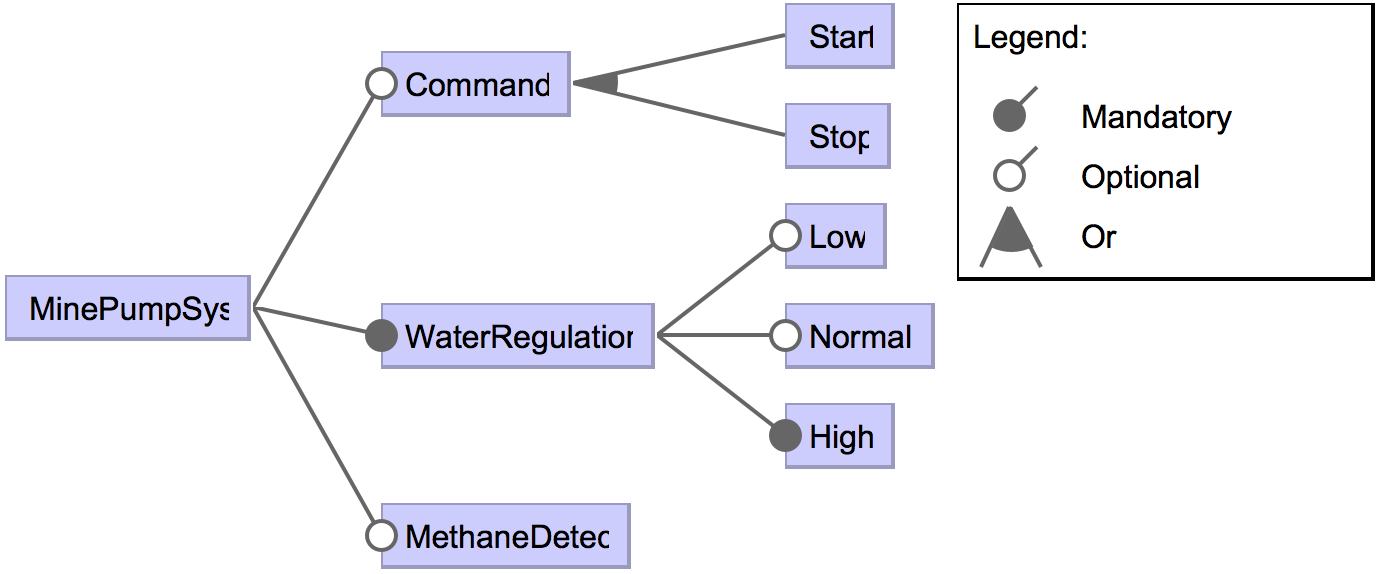
\includegraphics[width=95mm]{minepump-fm}
	\caption{Minepump feature model}
	\label{fig:minepumpfm}
\end{figure}

The Minepump model \cite{Classen2010b} represent a product line of pumps designed to keep a mine shaft clear of water and (optionally) avoid the danger of a methane explosion. Figure \ref{fig:minepumpfm} presents the feature model of the SPL. A pump has a water regulator that can detect the level of water in the shaft. It may be equipped with a methane detector and a command interface allowing to manually start and stop the pump. The FTS describing the behaviour of the pumps has 25 states and 41 transitions. 


%%%%%%%%%%%%%%%%%%%%%%%%%%%%%%%%%%%%%%%%%%%%%%%%%%%%%%%%%%%%%%
\section{Sferion\texttrademark landing symbology function}
%%%%%%%%%%%%%%%%%%%%%%%%%%%%%%%%%%%%%%%%%%%%%%%%%%%%%%%%%%%%%%

\label{sec:casestudy:sferion}

\begin{figure}
	\centering
	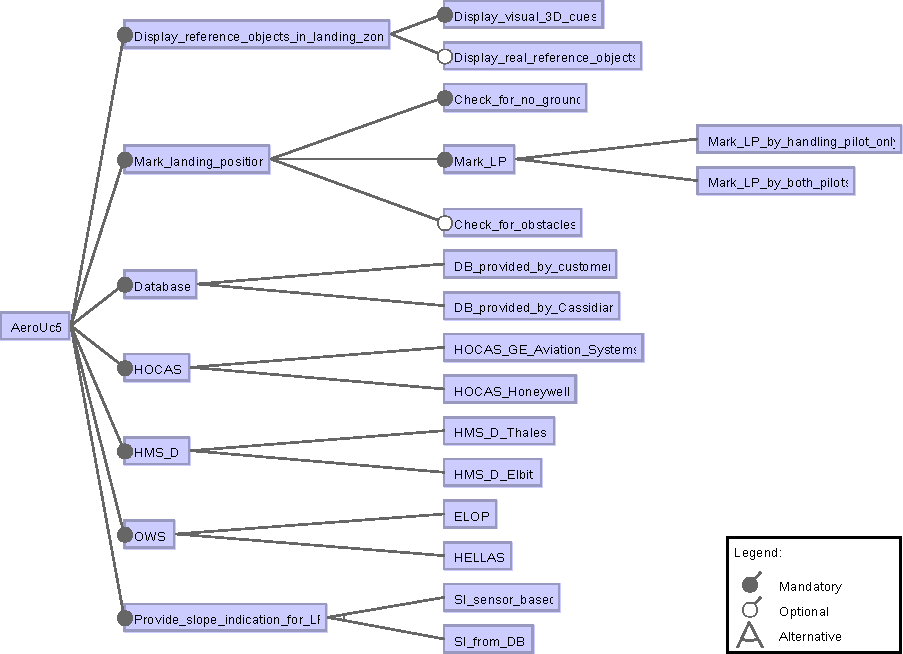
\includegraphics[width=0.98\textwidth]{aerouc5-fm}
	\caption{Sferion\texttrademark landing symbology function feature model}
	\label{fig:aerouc5fm}
\end{figure}

Sferion\texttrademark ~is an industrial situational awareness suite for helicopters flying in degraded visual environments \cite{Devroey2015a,sferion,Samih2014c}. The landing symbology function supports the pilot during the landing approach by marking the intended landing position on ground using a head-tracked Helmet Mounted Sight and Display (HMS/D) and Hands On Collective And Stick (HOCAS). Depending on the selected feature, the landing may be marked by the handling pilot only or by bots pilots. The spatial awareness is enhanced during the final landing approach by displaying 3D conformal visual cues on the helmet with optionally real reference of the object. The ground (and optionally obstacles) in the landing zone are detected and classified using a real-time Obstacle Warning System (OWS). Depending on the customer and the helicopter platform, the landing symbolog1y function may have different features (Figure \ref{fig:aerouc5fm}) selected: \textit{ELOP} or \textit{HELLAS} sensors for the \textit{OWS}; \textit{SI\_sensor\_based} or \textit{SI\_from\_DB} as slope indication provider for landing position; the Thales or Elbit HMS/D; the HOCAS from Honeywell or from Aviation Systems inc.; a database provided by the helicopter platform or a Cassidian database.

The models have been designed by engineers using MaTeLo \cite{matelo} tool, OVM and Matelo Product Line Management (MPLM) \cite{Samih2014b}. They have originally been presented by Samih et al. \cite{Samih2014c}. MaTeLo supports the description of statistical usage models by using hierarchical Markov chains. MaTeLo's usage model is a \gls{DTMC}, where the nodes represent the major states of the system and the transitions are labelled with the actions or operations of the SUT with their probability to be fired. In a DTMC, the transitions are tagged with a probability representing the likelihood, when we are in the starting state, to execute the transition, and the action performed when the transition is executed. Each action is associated with zero, one or more requirements. The variability is described using OVM (Orthogonal Variability Model), each variation point is associated to zero, one or more requirement(s). The mapping, encoded in MPLM, between the variation points and the usage model transitions is made through the requirements. MPLM and MaTeLo tools support the product-based test derivation approach.

We encoded the Sferion\texttrademark ~landing symbology function models using our formalisms: the usage model has been flattened to remove hierarchy (by hand in 1/2 day); the OVM model has been translated to a feature model (by hand in 1/2 day); and the mapping between features and behaviour has been encoded using an FTS, generated from the MaTeLo usage model, the OVM model and the MPLM mapping model (in 1 day).


%%%%%%%%%%%%%%%%%%%%%%%%%%%%%%%%%%%%%%%%%%%%%%%%%%%%%%%%%%%%%%
\section{WordPress, an open-source CMS}
%%%%%%%%%%%%%%%%%%%%%%%%%%%%%%%%%%%%%%%%%%%%%%%%%%%%%%%%%%%%%%

\label{sec:casestudy:wordpress}

WordPress \cite{wordpress} is a popular open-source \acrfull{CMS} used by more than 60 million websites \cite{Colao2012}. It includes a plugin architecture and a template system, allowing one to modify its behaviour by adding new functionalities (\ie plugins), or the rendering of the website (\ie themes), respectively. In February 2017, the WordPress database (\url{https://wordpress.org/}) counted 48,898 plugins and 4,462 (latest) themes. 

We reverse-engineered the feature models and the FTSs of two WordPress instances, AGE and Elsa portals, based on their Apache webserver log file. The \gls{AGE} website (\url{http://www.age-namur.be}) is the portal of the general student assembly of the University of Namur. It uses a dedicated WordPress instance and provided us a log file with 1,285,592 entries from May 2013 to March 2014. The European Law Students' Association (Elsa) of Louvain-la-Neuve  (\url{http://elsa-lln.be}) also uses a dedicated WordPress instance and provided us a log with 48,823 entries from February 2014 to the end of April 2014.

%---------------------------
\subsection{Feature model} 
%---------------------------

\label{subsec:wordpress:fm}

\begin{figure}
\centering
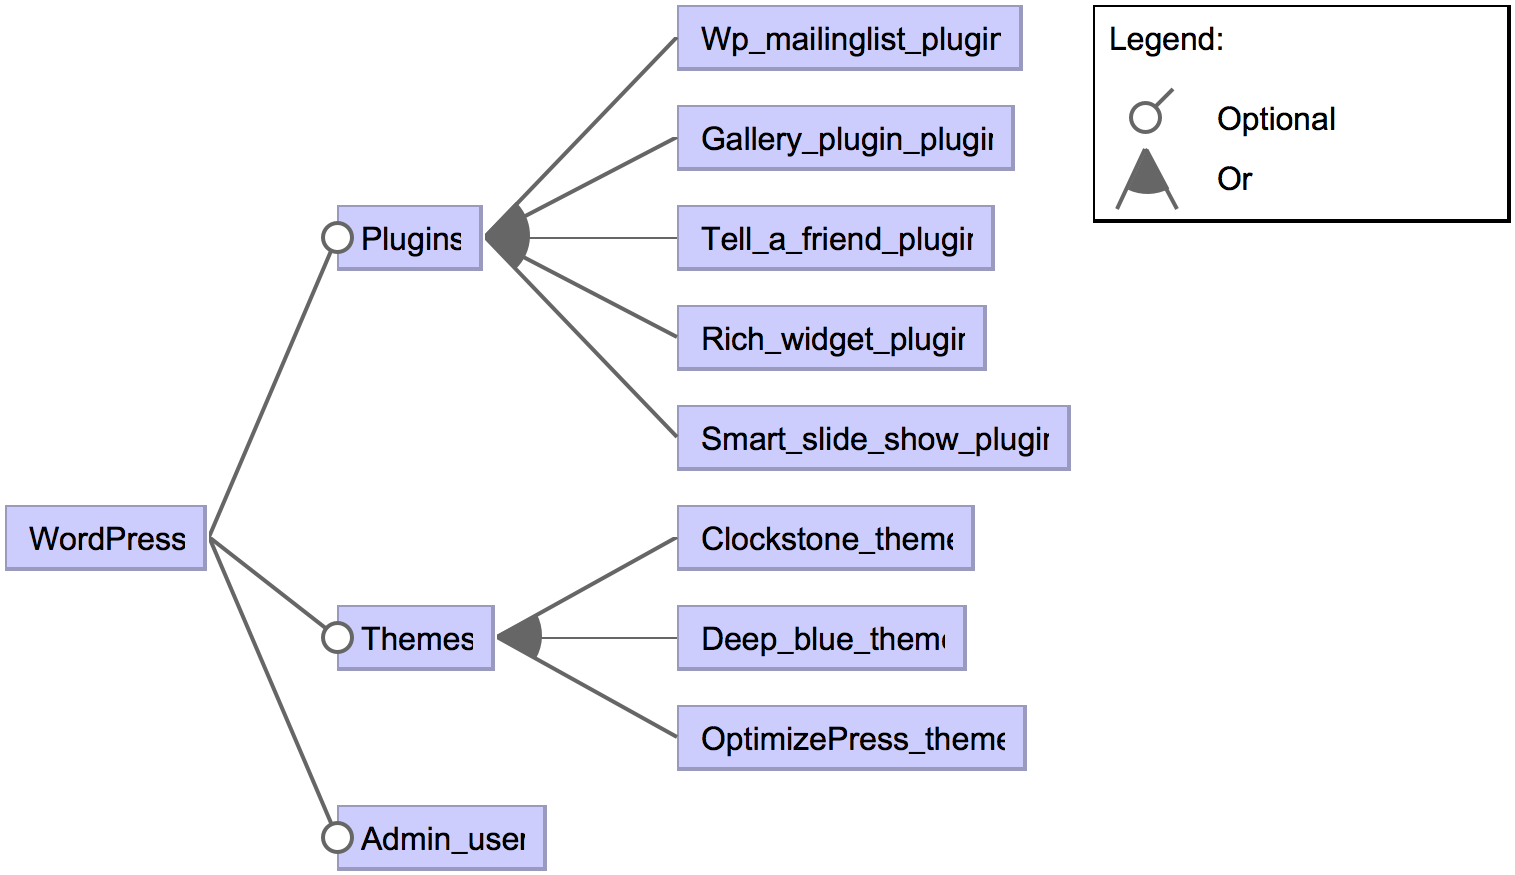
\includegraphics[width=100mm]{wordpress-simplified}
\caption{Simplified WordPress feature model}
\label{fig:wordpressfm}
\end{figure}

Our WordPress feature model has 3 optional core features: \textit{Plugins}, \textit{Themes}, and \textit{Admin\_user}. One configuration (\ie product) of the feature models represents the minimal instance needed to play a test suite. The \textit{Admin\_user} feature will be selected only if a test case requires to access the administration pages. 

To identify the plugins and themes used in the instances, we analysed the Apache webserver log entries. Each time an HTTP request is addressed to the server, one entry is created in the log file with the following format \cite{apacheserver}: the IP address of the visitor sending the request; a login if the visitor is identified on the system; the date and time of the request; the HTTP request itself, beginning with  GET, POST, \etc, followed by a URL and the protocol version; the status code sent back to the client; the size of the object returned to the client; the website the client reports having been referred from; and finally the information on the client's browser. For instance, a request to the \texttt{index.php} page of the WordPress instance from a Mozilla Firefox navigator will add the following entry in the log file:
%
\begin{lstlisting}[basicstyle=\footnotesize\ttfamily,frame=single,breaklines,columns=flexible]
66.155.40.250 - - [08/Nov/2013:11:38:11 +0100] "GET /index.php?p=potins&action=aimepas&id=135 HTTP/1.1" 200 708388 "-" "Mozilla/5.0 (Windows NT 6.1; WOW64; rv:25.0) Gecko/20100101 Firefox/25.0"
\end{lstlisting}
%
Plugins and themes resources are placed in specific folders on the webserver. This allows us to filter the URL of the log entries using the following regular expressions:
\begin{itemize}
\item \verb?.*/wp-content/plugins/([^/]+)/.*? to detect access to a plugin resource;
\item \verb?.*/wp-content/themes/([^/]+)/.*? to detect access to themes resources;
\item \verb?.*/wp-admin/.*? to detect that an administration page has been used.
\end{itemize}
The names of the plugins and themes appears right after the \texttt{plugins/} and \texttt{themes/} part of the URL (matched by the \verb?([^/]+)? part of the regular expression). Since the logs have been anonymized, we do not have the identification of the users and rely on the last regular expression to detect administrator accesses to the WordPress instance.

We ended up with two feature models: one with 45 features for the AGE WordPress instance, and one with 70 features for the Elsa WordPress instance. Figure \ref{fig:wordpressfm} presents a simplified version of the Elsa WordPress instance (AGE instance follows the same pattern).
The root feature \textit{WordPress} is decomposed in three optional sub-features: \textit{Admin\_user}, \textit{Themes}, and \textit{Plugins}. Each plugin or theme (resp.) appearing in a log entry will be a sub-feature of the \textit{Plugins} or \textit{Themes} (resp.) feature. 

Another approach to build the feature model would have been to mine the plugins and themes repository of WordPress. This would give a much larger feature model: more than 50,000 features. Since we are in behavioural model-based context, we seek to find incorrect behaviour in the product line. This incorrect behaviour may be caused by feature interaction or may have another root cause (\eg an error in the source code introducing faults in all the products). In order to select our test cases, we need a behavioural model of the SPL, which is derived from the Apache  Web server log. In this context, considering all the WordPress plugins and themes in the feature model has little meaning since only the behaviour of the plugins and themes activated in the running WordPress instances (appearing in the log) will appear in the behavioural model. This is why we consider only those plugins and themes as relevant for testing and add them in the feature models. 

Similarly, S\'anchez \etal \cite{Sanchez2013a,Sanchez2017} used a white box testing approach to test the Drupal CMS. They rely on documentation, source code, issue tracking system, and Git versioning repository to reverse engineer the system's feature model. Stress is put on product selection, whereas we focus on behaviour selection (at the product line level) in a black box approach. 

%---------------------------------------
\subsection{Featured transition system} 
%---------------------------------------

\label{subsec:wordpress:fts}

We reverse engineered the FTSs of the AGE and Elsa WordPress instances using a 2-gram (bigram) inference method \cite{Sprenkle2011a,Sprenkle2013}. This method uses a set of \emph{user sessions} (\ie sequences of HTTP requests) to generate a navigational model of a website. In the generated FTS, the states represents the last user request and the transitions represents the sequence between two requests. Transitions leading to a request identified as part of a plugin or a theme, or as accessible only by an administrator (using the regular expressions from the previous section) are labelled with the corresponding feature expression.

The $n$-gram inference method has been proposed by Sprenkle \etal \cite{Sprenkle2011a,Sprenkle2013} and used to test website in a black box fashion. They experiment the inference with different configurations and values of $n$ greater than 2 and found out that a small $n$ allows better diversity in the behaviours (ending up in more diverse test cases), and requires less sessions to reach growth stability of the model. Small $n$ also simplifies the generation and results in a more compact model. This motivates our choice to select 2-gram for the inference.


\paragraph{User sessions:}
%--------------------------

One user session corresponds to a sequence of HTTP requests, representing the sequence of pages consulted by the user. User sessions can be extracted from the Apache webserver log by grouping entries with the same IP address (assuming that one IP corresponds to one user) and logged within a same time frame. This means that two entries in a user session may not be distant by more than a maximal timeout (we arbitrarily choose to set a timeout of 3 minutes). If the timeout is reached, the next entry will be the first of a new user session.

To build the user sessions, we only consider some relevant elements of the HTTP request \cite{Sprenkle2013}. This allows to group behaviour of various users to identify common usage scenarios. Amongst the possible group of elements, we considered:
\begin{itemize}
\item \emph{Request type} and \emph{Resource} (RR), which uses the type of HTTP request (\eg PO\-ST or GET) and the resource name (\eg \texttt{/index.php}) for a user session element;
\item \emph{Request type}, \emph{Resource}, and \emph{parameters Names} (RRN), which also uses the HTTP request type and the name of the resource, but also the name of the parameters in the resource (\eg \verb|?p=&action=&id=|).
\end{itemize}

 
\paragraph{Bigram inference:}
%---------------------------

\begin{algorithm}[h]
	\KwIn{\textit{sessions}: the set of non empty user sessions}
	\KwOut{\textit{fts}: an FTS representing a navigational model}
	\Begin{
		$S = \{ s_0 \}$; $\Act = \emptyset$; $\trans = \emptyset$; $i=s_0$; $\gamma= \rightarrow (\rightarrow \bot)$ \; \nllabel{algo:bigram:line:init}
		\For{\textit{sess} $\in$ \textit{sessions} \nllabel{algo:bigram:line:mainloop}}{
			\textit{S.add(sess[0])}\; \nllabel{algo:bigram:line:sessioninit1}
			\textit{Act.add(req(sess[0]))} \; \nllabel{algo:bigram:line:sessioninit2}
			\textit{tr} = $s_0 \xrightarrow{\mathit{req}(\mathit{sess}[0])} \mathit{sess}[0]$\; \nllabel{algo:bigram:line:sessioninit3}
			\textit{trans.add(tr)}\; \nllabel{algo:bigram:line:sessioninit4}
			$\gamma = fLabels(\gamma, tr) $\; \nllabel{algo:bigram:line:sessioninit5}
			\For{$i \in [1;sess.size[$ \nllabel{algo:bigram:line:sessionloop}}{
				\textit{S.add(sess[i])}\;  \nllabel{algo:bigram:line:addstate}
				\textit{Act.add(req(sess[i]))}\; \nllabel{algo:bigram:line:addaction}
				\textit{tr} = \textit{sess[i-1]} $\xrightarrow{\mathit{req}(\mathit{sess}[i])}$ \textit{sess[i]}\; \nllabel{algo:bigram:line:addtransition}
				\textit{trans.add(tr)}\; 
				$\gamma$ = \textit{fLabels(}$\gamma$\textit{, tr, sess[i])} \; \nllabel{algo:bigram:line:addlabels}
	  		}
			$Act.add(req(s_0))$\; 
			$trans.add(sess[sess.size - 1] \xrightarrow{req(s_0)} s_0)$\;	 \nllabel{algo:bigram:line:addfinaltransition}
	  	}		
	  	$\fts = (S, \Act, \trans, i, \mathit{fm}(\mathit{sessions}), \gamma)$\; \nllabel{algo:bigram:line:ftsinit}
  		\Return $fts$\;
	}
	\caption{WordPress bigram FTS building}
 \label{algo:bigram}
\end{algorithm}

Using a bigram inference, the next state only depends on the current state of the system. As a consequence, user session entries are considered two by two: the last user request, which is the current state, and the next request of the user, which is the next state of the system.

Algorithm \ref{algo:bigram} presents the bigram inference of the FTS for a WordPress instance, based on a set of user sessions. The elements of the FTS are initialised at line \ref{algo:bigram:line:init}. For each session (line \ref{algo:bigram:line:mainloop}), the sequence of requests enriches the model: sessions starts from a virtual state $s_0$ and the first sequence adds a transition from this state to a new state corresponding to the first element of the sequence (lines \ref{algo:bigram:line:sessioninit1} to \ref{algo:bigram:line:sessioninit3}); transitions are labelled with actions representing the request of another page (lines \ref{algo:bigram:line:sessioninit2} and \ref{algo:bigram:line:addaction}); and each new transition is labelled with a feature expression (lines \ref{algo:bigram:line:sessioninit5} and \ref{algo:bigram:line:addlabels}).
%
This feature expression corresponds to the conjunction of the previous feature expression if there is one or true otherwise, and the  name of a plugin, a theme, or the administrator user if the requested resource matches one of the corresponding regular expression from section \ref{subsec:wordpress:fm}. Function \textit{fLabels} enriches $\gamma$ definition, based on its previous definition and the given transition. 
%
This process iterates for each request in the sequence (line \ref{algo:bigram:line:sessionloop}), the starting state corresponding to the target state of the previous iteration. Finally, each sequence terminates by a special action \textit{req}$(s_0)$, resetting the system, and ends in the virtual state $s_0$ (line \ref{algo:bigram:line:addfinaltransition}). The algorithm returns an FTS with the inferred navigational model and a feature diagram build using the method described in section \ref{subsec:wordpress:fm} (line \ref{algo:bigram:line:ftsinit}). We implemented Algorithm \ref{algo:bigram} in an open source tool: Yet Another Model Inference tool (YAMI), available at \url{https://github.com/xdevroey/yami}.

We built four FTSs: two using Request type and Resource (RR) parts of the URLs as sequence elements in the user sessions (\emph{AGE-RR} with 772 states and 6,639 transitions, and \emph{Elsa-RR} with 384 states and 1,214 transitions), and two using Request type, Resource, and parameter Names (RRN) parts of the URLs (\emph{AGE-RRN} with 1,101 states and 10,960 transitions, and \emph{Elsa-RRN} with 615 states and 1,771 transitions). The process took 3 seconds to process the 3,964 sessions of the Elsa models (average session size=9.57, $\sigma$=46.73) and 54 second to build the 147,173 sessions of the AGE models (average session size=5.10, $\sigma$=61.04) on a Ubuntu Linux machine (Linux version 3.13.0-65-generic, Ubuntu 4.8.2-19ubuntu1) with an Intel Core i3 (3.10GHz) processor and 4GB of memory.


%%%%%%%%%%%%%%%%%%%%%%%%%%%%%%%%%%%%%%%%%%%%%%%%%%%%%%%%%%%%%%
\section{Claroline, a course management system}
%%%%%%%%%%%%%%%%%%%%%%%%%%%%%%%%%%%%%%%%%%%%%%%%%%%%%%%%%%%%%%

\label{sec:casestudy:claroline}

The instance of Claroline at University of Namur\footnote{\url{http://webcampus.unamur.be}} is the main communication channel between students and lecturers and is used by approximately 7000 users. Students may register to courses and download documents, receive announcements, submit their assignments, perform online exercises, \etc 
Claroline is a configurable system \cite{Cohen2008}. Contrary to classical SPL, the selection of the features does not occur during the development of the software (at design time in a SPL lifecycle) \cite{Pohl2005}, but during its execution (at runtime). Thus, a product can dynamically evolve while the system is running: this requires the system architecture to be able to accommodate evolutions, by following plugin-based or component-based architectural styles. Thanks to the versatility of the feature concept \cite{Classen2008}, it is possible to represent design time and runtime product using the same formalism (FM), as product semantics is ultimately given through the mapping with the FTS. In the Claroline case, features represent installation parameters. A product represents a running Claroline instance with a minimal set of data.  

%---------------------------
\subsection{Feature model} 
%---------------------------

\label{sec:casestudy:claroline:fm}

\begin{figure}
\centering
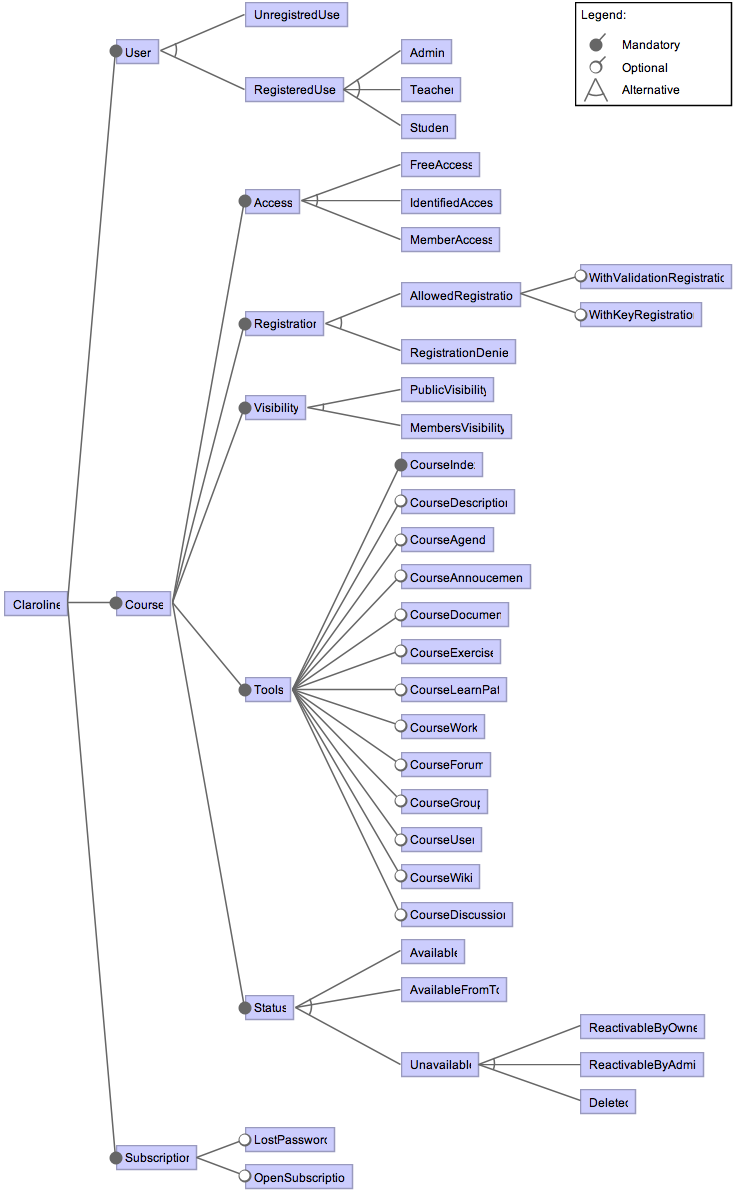
\includegraphics[height=0.95\textheight]{claroline-fm}
\caption{Claroline feature model}
\label{fig:clarolinefm}
\end{figure}

We manually built the \gls{FM} from the Claroline documentation and from inspection of a locally installed Claroline instance (Claroline 1.11.7) in approximately 3 days (by one person). The FM in Fig. \ref{fig:clarolinefm} (additional constraints have been omitted) describes Claroline with three main features: \textit{User}, \textit{Course} and \textit{Subscription}. \textit{Subscription} may be open to everyone (\textit{opt} \textit{OpenSubscription}) and may have a password recovery mechanism (\textit{opt} \textit{LostPassword}). 

\textit{User} corresponds to the different possible user types provided by default with a basic Claroline installation: unregistered users (\textit{UnregisteredUser}) who may access courses open to everyone and registered users (\textit{RegisteredUser}) who may access different functionalities of the courses according to their privilege level (\textit{Student}, \textit{Teacher} or \textit{Admin}). The last main feature, \textit{Course}, corresponds to the page dedicated to a course where students and teacher may interact.

A course has a status (\textit{Available}, \textit{AvailableFromTo} if the course is available only during a specific period, or \textit{Unavailable}), may be publicly visible (\textit{PublicVisibility}) or not (\textit{MembersVisibility}), may authorize registration to identified users (\textit{AllowedRegistration}) or not (\textit{RegistrationDenied}) and may be accessed by everyone (\textit{FreeAccess}), identified users (\textit{IdentifiedAccess}) or members of the course only (\textit{MembersAccess}). Moreover, a course may have a list of tools (\textit{Tools}) used for different teaching purposes, \eg an agenda (\textit{opt} \textit{CourseAgenda}), an announcement panel (\textit{opt} \textit{CourseAnnoucements}), a document download section where lecturers may post documents and students may download them (\textit{opt} \textit{CourseDocument}), an online exercise section (\textit{opt} \textit{CourseExercise}).
 
Since we are in a testing context, one product of the FM does not represent a complete Claroline instance, but the minimal instance needed to play a test suite. Basically, it maps to a Claroline instance with one particular user and one particular course.
This is similar to the technique presented by Segura et al. \cite{Segura2014} used to represent the testing entry domain of a e-commerce web site.
In order to represent a complete Claroline instance (with all its users and courses), we need to introduce cardinalities \cite{Michel2011} on the \textit{User} and  \textit{Course} features in order to have multiple users and multiple courses. Eventually we obtained a FM with 44 features.

%---------------------------------------
\subsection{Featured transition system} 
%---------------------------------------

\label{sec:casestudy:claroline:fts}

Regarding the \gls{FTS}, we also used a bigram inference method (see section \ref{subsec:wordpress:fts}) on a 5.26 Go Apache webserver log with 45,210,987 entries from January 2013 to September 2013. Contrary to the AGE and Elsa models, we only consider the resource names in the user sessions. This simplification is coherent with our testing context where the FM is used to map a Claroline instance with one particular user and one particular course.

Finally, lines \ref{algo:bigram:line:sessioninit5} and \ref{algo:bigram:line:addlabels} have been omitted in algorithm \ref{algo:bigram} for the Claroline FTS and transitions have been subsequently tagged manually (in the produced model) with feature expressions based on the knowledge of the system (via the documentation and the local Claroline instance). As for the WordPress models, we added an initial state $s_0$, but made all states in the FTS accessible from $s_0$. This allows to simulate a web browser access both to the root page or directly to a sub-page of the website (\eg from a direct link sent in an email), which is a very common way to access Webcampus. The final FTS consists of 106 states and 2053 transitions and has been built in approximately 4 days (by the author).


%%%%%%%%%%%%%%%%%%%%%%%%%%%%%%%%%%%
\section{Models characteristics}
%%%%%%%%%%%%%%%%%%%%%%%%%%%%%%%%%%%

\label{sec:casestudy:characteristics}

\begin{table}
\centering
\caption{Characteristics of the \glspl{FTS} of the different case studies}
\begin{tabularx}{0.90\textwidth}{l r r r >{\raggedleft\arraybackslash}X >{\raggedleft\arraybackslash}X >{\raggedleft\arraybackslash}X}
\hline
\textbf{\small{Model}}	& \textbf{\small{States}}	& \textbf{\small{Trans.}}	& \textbf{\small{Act.}} & \textbf{\small{Avg. deg.}}	& \textbf{\small{BFS height}}	& \textbf{\small{Back lvl tr.}} \\
\hline 
\small{S.~V.~Mach.}		& \small{9}		& \small{13}		& \small{14}		& \small{1.44}		& \small{5}		& \small{3} \\
\small{C.~P.~Term.}		& \small{11}		& \small{17}		& \small{16}		& \small{1.54}		& \small{7}		& \small{4} \\
\small{Minepump}			& \small{25}		& \small{41}		& \small{23}	 	& \small{4.64}		& \small{15}		& \small{9} \\
\small{Sferion\texttrademark}	& \small{25}		& \small{46}		& \small{12}		& \small{1.84}		& \small{16}		& \small{14} \\
\small{AGE-RR}			& \small{772}	& \small{6,639}	& \small{772} 	& \small{8.60}		& \small{328}	& \small{408} \\
\small{AGE-RRN}			& \small{1,101}	& \small{10,960}	& \small{1,101} 	& \small{9.96}		& \small{426}	& \small{662} \\
\small{Elsa-RR}			& \small{384} 	& \small{1,214}	& \small{384} 	& \small{3.16}		& \small{194}	& \small{174} \\
\small{Elsa-RRN}			& \small{615}	& \small{1,771}	& \small{615} 	& \small{2.88}		& \small{369}	& \small{289} \\
\small{Claroline}		& \small{106}	 & \small{2,055}	& \small{106} 	& \small{19.37}		& \small{1}		& \small{105} \\
%Random 1			& 15000	& 20488	& 150 	& 1.37		& 11865	& 4899 \\
%Random 2			& 15000	& 20488	& 210 	& 1.37		& 11865	& 4899 \\
%Random 3			& 15000	& 20488	& 300 	& 1.37		& 11865	& 4899 \\ %ts-62e92b35
%Random 4			& 15000	& 20488	& 61 	& 1.37		& 11865	& 4899 \\
%Random 5			& 15000	& 20488	& 270 	& 1.37		& 11865	& 4899 \\
%Random 6			& 15000	& 20488	& 30 	& 1.37		& 11865	& 4899 \\
%Random 7			& 10000	& 13652	& 120 	& 1.37		& 7924	& 3303 \\ %ts-f5e050b4
%\small{Random}			& \small{10,000}	& \small{13,652}	& \small{120} 	& \small{1.37}		& \small{7,924}	& \small{3,303} \\ %ts-f5e050b4
\hline
\end{tabularx}
\label{tab:models:fts}
\end{table}

Table \ref{tab:models:fts} details the employed FTS models. For each model, we measure: the number of states (\emph{States}); the number of transitions (\emph{Trans.}); the number of actions (\emph{Act.}); the average degree of the different states that correspond to the average number of incoming/outgoing transitions per state (\emph{Avg. deg.}), computed as the number of transitions divided by the number of states; the maximal number of states between the initial state and another state when traversing the \gls{FTS} in breadth-first search (\emph{BFS height}); the number of transitions starting from a state and ending in another state with a lower level when traversing the FTS in breadth-first search (\emph{Back lvl tr.}).

\begin{table}
\centering
\caption{Characteristics of the \glspl{FM} of the different case studies}
\begin{tabularx}{0.90\textwidth}{l r >{\raggedleft\arraybackslash}p{1.5cm} >{\raggedleft\arraybackslash}p{1.2cm} >{\raggedleft\arraybackslash}p{1.2cm} >{\raggedleft\arraybackslash}X}
\hline
\textbf{\small{Model}}	& \textbf{\small{Feat.}}	& \textbf{\small{Common feat.}}	& \textbf{\small{Mand. feat.}} & \textbf{\small{Opt. feat.}}	& \textbf{\small{Prod.}} \\
\hline 
\small{S.~V.~Mach.}		& \small{9}		& \small{3}		& \small{2}		& \small{2}			& \small{24,000} \\
\small{C.~P.~Term.}		& \small{21}		& \small{4}		& \small{4}		& \small{2}			& \small{4,774} \\
\small{Minepump}			& \small{9}		& \small{3}		& \small{2}	 	& \small{4}			& \small{32,000} \\
\small{Sferion\texttrademark}	& \small{25}		& \small{13}		& \small{10}		& \small{2}		& \small{64,000}	 \\
\small{AGE-RR}			& \small{45}		& \small{1}		& \small{0} 		& \small{3}			& \small{4.3980e+12} \\
\small{AGE-RRN}			& \small{45}		& \small{1}		& \small{0} 		& \small{3}			& \small{4.3980e+12} \\
\small{Elsa-RR}			& \small{70} 	& \small{1}		& \small{0} 		& \small{3}			& \small{1.4757e+20} \\
\small{Elsa-RRN}			& \small{70} 	& \small{1}		& \small{0} 		& \small{3}			& \small{1.4757e+20} \\
\small{Claroline}		& \small{44}		& \small{10}		& \small{9} 		& \small{16}			& \small{5.4067e+06} \\
\hline
\end{tabularx}
\label{tab:models:fm}
\end{table}

Table \ref{tab:models:fm} presents the main characteristics of the \glspl{FM} of the different cases studies. Those characteristics have been computed using SPLAR \cite{Mendonca2010}, the library used by the Software Product Lines Online Tools (SPLOT) \cite{Mendonca2009} to perform its analyses. For each FM, it gives the number of features (\emph{Feat.}), the number of features common to all products (\emph{Common feat.}), the number of mandatory (\emph{Mand. feat.}) and optional (\emph{Opt. feat.}) features in the model, and the number of possible products (\emph{Prod.}) for this FM.


%%%%%%%%%%%%%%%%%%%%%%%%%%%%%%%%%%%
\section{Additional random LTS models}
%%%%%%%%%%%%%%%%%%%%%%%%%%%%%%%%%%%

\label{sec:casestudy:random}

Additionally to the previously presented case studies, we generated four random LTS models (\textit{Random 1-4}). Those models are used during the assessment of our mutation analysis approaches in Sections \ref{sec:experiment:fmmexec} and \ref{sec:experiment:mutequiv}. 

In his work, Pel\'anek \cite{Pelanek2008a,Pelanek2004a,Pelanek2008} measured different properties (like the ones from Table \ref{tab:models:fm}) of real world software system LTSs. The idea behind the procedure we used to generate those LTSs is to mimic those properties:
%
\begin{enumerate}
\item we generate a set of random graphs (basically directed arcs and nodes) and compute the different measures (as the ones defined in Table \ref{tab:models:fts}) on them;
\item we select those graphs that are likely to represent a real system, \ie those having a small average degree, a large BFS height and a small number of back level edges (in this order);
\item we apply a random labelling multiple times and computed the occurrence probability, \ie the probability of the labels to obtain a set of randomly generated LTSs;
\item we select the LTS that had the following properties: the probability of the most occurring label in the LTS was less than or equal to $6\%$, and the cumulated probability of the 5 most frequently occurring labels was less than or equal to $20\%$;
\item we arbitrarily set the initial state to the first state in the graph.
\end{enumerate}
%
The characteristics of the four generated random models are presented in Table \ref{tab:models:random}.

\begin{table}
\centering
\caption{Characteristics of the random LTSs}
\begin{tabularx}{0.90\textwidth}{l r r r >{\raggedleft\arraybackslash}X >{\raggedleft\arraybackslash}X >{\raggedleft\arraybackslash}X}
\hline
\textbf{\small{Model}}	& \textbf{\small{States}}	& \textbf{\small{Trans.}}	& \textbf{\small{Act.}} & \textbf{\small{Avg. deg.}}	& \textbf{\small{BFS height}}	& \textbf{\small{Back lvl tr.}} \\
\hline 
%S.~V.~Mach.	& 9			& 13		& 14	& 1.44		& 5			& 3 \\%svm
%C.~P.~Term.	& 16		& 17		& 15	& 1.55		& 7		& 4 \\%cpterminal
%Minepump	& 25		& 41		& 23	& 4.64		& 15		& 9 \\%minepump
%Claroline	& 106		& 2,055		& 106 	& 19.37		& 1			& 105 \\%claroline
%Elsa-RR		& 384 		& 1,214		& 384 	& 3.16		& 194		& 174 \\%elsaRR
%Elsa-RRN	& 615		& 1,771		& 615 	& 2.88		& 369		& 289 \\%elsaRRN
%AGE-RR		& 772		& 6,639		& 772 	& 8.60		& 328		& 408 \\%ageRR
%AGE-RRN		& 1,101		& 10,960	& 1,101	& 9.96		& 426		& 662 \\%ageRRN
Random 1	& 10,000	& 13,652	& 120 	& 1.37		& 7,924		& 3,303 \\ %ts-f5e050b4
Random 2	& 15,000	& 20,488	& 300 	& 1.37		& 11,865	& 4,899 \\ %ts-62e92b35
Random 3	& 15,000	& 20,488	& 210 	& 1.37		& 11,865	& 4,899 \\ %ts-51d69eaf
Random 4	& 15,000	& 20,488	& 150 	& 1.37		& 11,865	& 4,899 \\ %ts-6cc2cfa6
\hline
\end{tabularx}
\label{tab:models:random}
\end{table}


%%%%%%%%%%%%%%%%%%%%%%%%%%%%%%%%%%%
\section{Threats to validity}
%%%%%%%%%%%%%%%%%%%%%%%%%%%%%%%%%%%

\label{sec:casestudy:threats}

The case studies presented in this chapter are used (in Chapter \ref{chap:assessment}) to assess test case selection and mutation analysis.  
We cannot guarantee that those case studies are representative of all the existing systems. In order to mitigate the validity threats, we choose different kinds of systems, coming from different sources: embedded systems designed by an engineer and Web-based applications where the model has been reverse-engineered from a running instance. The random models were built from a set of generated LTSs in order to match the real system state-space measures.


%%%%%%%%%%%%%%%%%%%%%%%%%%%%%%%%%%%
\section{Wrap up}
%%%%%%%%%%%%%%%%%%%%%%%%%%%%%%%%%%%

In the remainder of this thesis, we consider different case studies, representing different kinds of systems, and coming form different sources. Our largest \glspl{FTS} represent the usage of \emph{Web applications}: WordPress (AGE-RR, AGE-RRN, Elsa-RR, Elsa-RRN) and Claroline.
%
The other models represent \emph{embedded systems} with a more constrained behaviour. 
%
Four additional randomly generated LTS models, that mimic properties of real world system, are used during mutation analysis assessments.





